%----------------------------------------------------------------------------------------
%	PACKAGES AND OTHER DOCUMENT CONFIGURATIONS
%----------------------------------------------------------------------------------------
\documentclass[11pt,a4paper]{article}

\usepackage[utf8]{inputenc} % to encode the document so that we can use more caracters (like Latin ones)
\usepackage[T1]{fontenc} % to encode the document so that we can use more caracters (like Latin ones)
\usepackage[english]{babel} % to write in English

\usepackage{geometry} % the paper's format and marges
\geometry{hmargin=2.3cm,vmargin=1.7cm}

\usepackage{titling} % to put the title where I want

% maths packages
\usepackage{mathtools}
\usepackage{amsmath,amsbsy}
\usepackage{bm}
\usepackage{bigints}
\usepackage{stmaryrd}
\usepackage{amsfonts}

% graphs packages
\usepackage{graphicx}
\usepackage{float}
\usepackage{caption}
\usepackage{subcaption}
\usepackage{wrapfig,epsfig}

\usepackage{color}

\newtheorem{theorem}{Theorem}[section]
\newtheorem{lemma}[theorem]{Lemma}
\newtheorem{proposition}[theorem]{Proposition}
\newtheorem{corollary}[theorem]{Corollary}

\newenvironment{proof}[1][Proof]{\begin{trivlist}
		\item[\hskip \labelsep {\bfseries #1}]}{\end{trivlist}}
\newenvironment{definition}[1][Definition]{\begin{trivlist}
		\item[\hskip \labelsep {\bfseries #1}]}{\end{trivlist}}
\newenvironment{example}[1][Example]{\begin{trivlist}
		\item[\hskip \labelsep {\bfseries #1}]}{\end{trivlist}}
\newenvironment{remark}[1][Remark]{\begin{trivlist}
		\item[\hskip \labelsep {\bfseries #1}]}{\end{trivlist}}

\newcommand{\qed}{\nobreak \ifvmode \relax \else
	\ifdim\lastskip<1.5em \hskip-\lastskip
	\hskip1.5em plus0em minus0.5em \fi \nobreak
	\vrule height0.75em width0.5em depth0.25em\fi}

\usepackage{vmargin}
\setmarginsrb{0.5cm}{0.5cm}{1cm}{1cm}{0cm}{0cm}{0cm}{0cm}

\usepackage[final]{pdfpages}

\usepackage{algorithm}
\usepackage{algorithmic}
%----------------------------------------------------------------------------------------
%DOCUMENT
%----------------------------------------------------------------------------------------

\begin{document}
\newcommand{\heavi}{h_{\epsilon}}
\newcommand{\heaviP}{h'_{\epsilon}}
\newcommand{\heaviPP}{h''_{\epsilon}}

\newcommand{\Math}[1]{\textcolor{red}{\textbf{#1}}}

\newcommand{\intO}{\int_{\Omega}}
\newcommand{\bigintO}{\bigint_{\Omega}}
\newcommand{\accDeuxcol}[1]{\left\{\begin{array}{ll}#1\end{array}\right.}
\newcommand{\accUnecol}[1]{\left\{\begin{array}{l}#1\end{array}\right.}

\newcommand{\stilde}{\tilde{s}}
\begin{center}
	\textbf{Optimisation de la largeur entre les droites avec contrainte de température - 21/02/2018}
\end{center}


\section*{Modèle et objectif}

On s'intéresse à la construction d'une pièce rectangulaire $\Omega$ par méthode SLM ($\partial\Omega=\Gamma_N\cup\Gamma_D,\,\,\Gamma_N\cap\Gamma_D$). On souhaite donc faire passer une sourc de chaleur le long d'une trajectoire prédéfinie afin de faire fusionner le lit de poudre. Cependant, il ne faut pas que la température puisse être trop élevée sous peine de créer des contraintes résiduelles thermiques qui nuiraient à la qualité de la pièce. 

\vspace{0.5cm}

Le travail présenté dans ce document consiste à, ayant choisi une trajectoire de type ligne droite pour le laser, optimiser la distance entre les lignes afin de fusionner la poudre ($\forall x\in\Omega,\,\,\exists t\in[0,t_F]\,\,\textrm{tel\,\,que}\,\,T(x,t)>T_{phase}$) tout en maitrisant la température dans le solide ($\forall x\in\Omega,\forall t\in [0,t_F],\,\,T(x,t)<T_{sup}$).

\subsection*{Modélisation thermique}
On commence par introduire le modèle thermique utilisé ici. Il est semblable à celui utilisé dans l'article de Lukas. On rajoute ici de la diffusion car notre modèle est seulement 2D et on veut tout de même modéliser la perte de chaleur dans les couches inférieures. Les conditions aux limites sont les conditions de Dirichlet car autour du solide, on a uniquement de la poudre qui est adiabatique. On cherche un champ de température $T(x,t) : [0,t_F]\times D \rightarrow \mathbb{R}$ tel que :

\begin{equation}
\label{eq:heatEq}
\accDeuxcol{
\rho\partial_t T+\frac{\lambda}{ep_{car}^2}(T-T_{ini}) -div(\lambda\nabla T)=Q & \textrm{in\,}(0,t_F)\times D \\
T=T_{ini} & \textrm{in\,}(0,t_F)\times \partial\Omega \\
T(0)=T_{ini} & \textrm{in} \Omega
}
\end{equation}

Le solide et la poudre ont des valeurs différentes pour les parametres physiques suivants (en notant $\chi_{solid}$ la fonction caractéristique du solide):
\begin{equation}
\begin{aligned}
\rho=\rho_{solid}*\chi_{solid}+\rho_{powder}*(1-\chi_{solid}) \\
\lambda=\lambda_{solid}*\chi_{solid}+\lambda_{powder}*(1-\chi_{solid}) \\
\beta=\beta_{solid}*\chi_{solid}+\beta_{powder}*(1-\chi_{solid}) \\
\end{aligned}
\end{equation}

\subsection*{Trajectoire de la source}
On considère une trajectoire en ligne droite comme sur le schéma ci-dessous (Figure XXX). On estime que la vitesse du laser est constante et égale à 1. On prend pour pas de temps $\delta t=2*\delta x$. La source est modélisée par une gaussienne centrée en un point (Figure XXX). 


%\begin{figure}[H]
%	\begin{minipage}{0.45\textwidth}
%		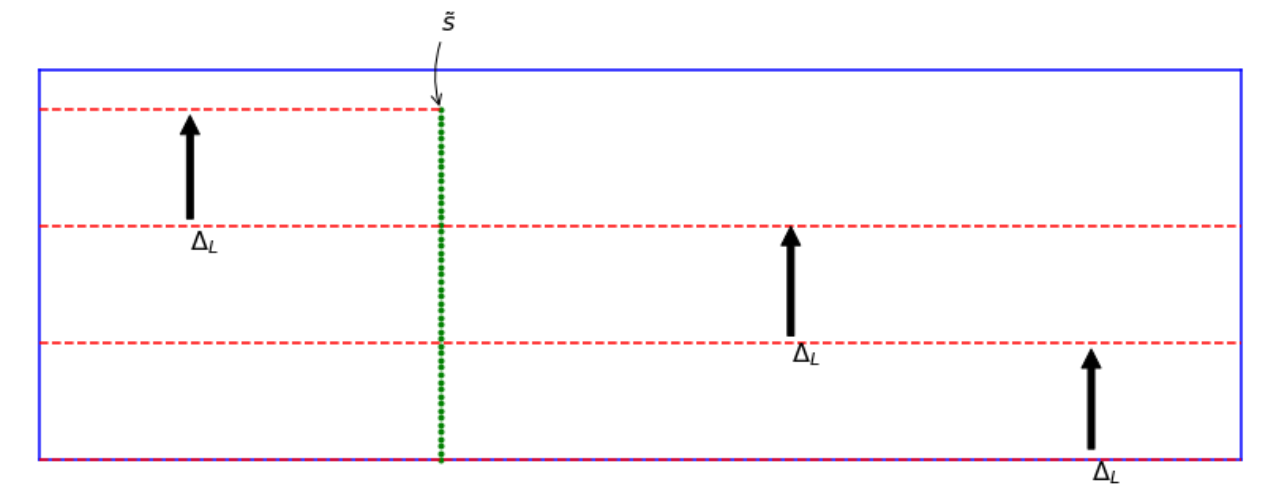
\includegraphics[width=0.9\textwidth]{trajectoire}
%	\end{minipage}
%	\begin{minipage}{0.45\textwidth}
%		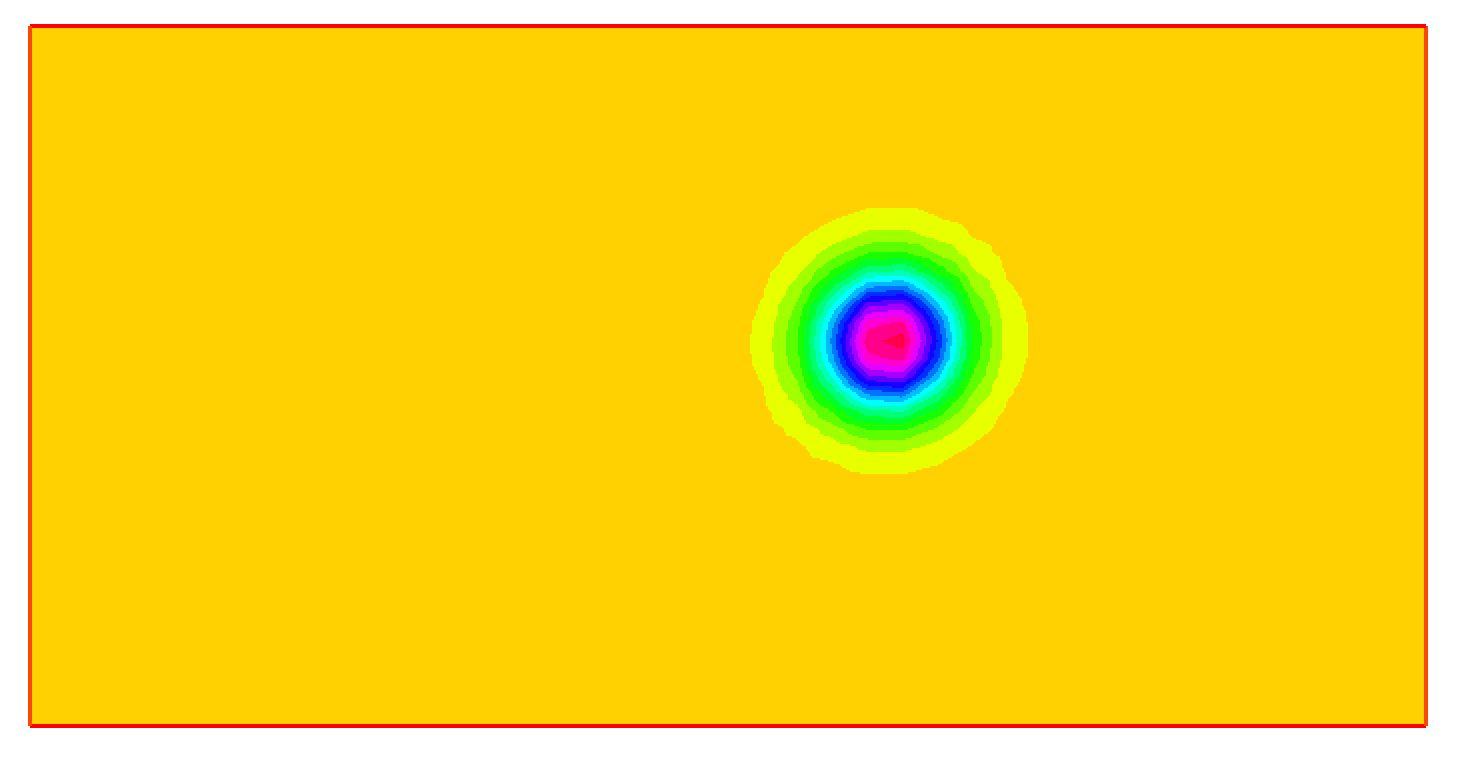
\includegraphics[width=0.9\textwidth]{source}
%	\end{minipage}
%\end{figure}

On modélise dans un premier temps le temps pour changer de ligne comme nul. De plus, on considère un temps final $t_F$, temps nécessaire pour effectuer toute la trajectoire comme constant. On estime que, que les lignes droites soient "dans le domaine de calcul ou non", la source va y passer. Ainsi, on décorrèle le temps final de la trajectoire de lasage ce qui permet de le considérer comme un paramètre fixe lors de l'optimisation (Figure XXX). \\
Afin de modéliser l'arret de la source lorsqu'on sort de la zone de travail, on choisit de multiplier la source à une fonction de heaviside qui s'annule lorsque le laser sort de la zone de travail. Ainsi, la zone continue de parcourir "pour de faux" des lignes hors du domaine de travail sans perturber la thermique. Cette approche induit deux discontinuités différentes : 
\begin{itemize}
	\item discontinuité de la source avec la fonction de heaviside.
	\item discontinuité des paramètres de la fonction de heaviside : le temps $t_s$ auquel la source sort du domain de travail et s'éteint est fortement discontinu par rapport à l'écartement entre les lignes $\Delta L$ (il s'agit même d'une fonction en escaliers).  
\end{itemize}

On peut éliminer la deuxième discontinuité en introduisant une deuxième variable, $\tilde{s}$ à optimiser et qui représente la longueur parcourue par le laser. Cette longueur n'est pas nécessairement proportionnelle à la longueur d'une ligne et donc on peut estimer que la source doit s'éteindre au milieu de la dernière ligne. La source est alors modélisée par une gaussienne centrée en un point mouvant, dépendant du temps et de l'écartement entre les lignes $\Delta L$ et d'une fonction de heaviside qui vaut 0 lorsque l'on a "dépassé l'abscisse curviligne finale $\tilde{s}$" : $1_{tV<\tilde{s}}$. On a toujours ici la discontinuité de la source avec la fonction de heaviside. Cependant, l'abscisse curviligne est, elle, continue, ce qui nous évite la deuxième discontinuité.


\section*{Theorie}
\subsection*{Probleme}

On veut minimiser les endroits n'ayant pas subi de changement phase tout en ne dépassant jamais une valeur seuil de la température ($T_{sup}$), en tout point et en tout instant de fabrication.

Les paramètre d'optimisation sont :
\begin{itemize}
	\item la distance entre deux lignes de parcours du laser $\Delta L$. On borne $\Delta L$ par 0 et par la largeur de la pièce ($\Delta L\in[0,L_{max}]$).
	\item l'"abscisse curviligne" finale $\tilde{s}$ qui détermine l'arret de la source. On borne $\tilde{s}$ par 0 et par un nombre de ligne maximal (déterminé par le temps final constant $t_F$ choisi) multiplié par le temps de parcours d'une seule ligne. \Math{A vérifier quand même... ça ou le temps qu'on reste sur le rectangle? -> je dirais peu importe}
\end{itemize}
 
\subsection*{Equation de la chaleur}

On pose $\tilde{T}=T-T_{ini}$ (i.e. $T=\tilde{T}+T_{ini}$). On a alors, d'après l'équation \ref{eq:heatEq} (l'arret de la source est modélisée par la fonction source $Q$ elle même. On écrit donc bien l'équation jusqu'à $t_F$ fixé) :

\begin{equation}
\label{eq:ChaleurTilde}
\accDeuxcol{
\Big(\rho\partial_t \tilde{T}+\frac{\lambda}{ep_{car}^2} \tilde{T}-div(\lambda\nabla \tilde{T})\Big)=Q(\Delta L,\tilde{s})& \textrm{in\,}(0,t_F))\times D \\
\tilde{T}=0 & \textrm{in\,}(0,t_F)\times \Gamma_D \\
\tilde{T}(0)=0 & \textrm{in} \Omega
}
\end{equation}




Le problème variationnel lié à la chaleur est alors le suivant :

trouver $\tilde{T}\in V=\{w\in H^1([0,t_M],\Omega) \textrm{tel\,\,que} \,\,w|_{\Gamma_D}=0\}$ tel que

\begin{equation}
\label{eq:pbVarChaleurTF}
\begin{aligned}
\forall v\in V,\,\forall t\in[0,t_M], \qquad\int_{\Omega}\rho\partial_t \tilde{T}v+\frac{\lambda}{ep_{car}^2} \tilde{T}v dx+\int_{\Omega}\lambda\nabla \tilde{T}\nabla vdx-\int_{\Omega}Q(\Delta L,\tilde{s})vdx=0
\end{aligned} 
\end{equation}

\subsection*{Changement de phase}
On souhaite ici que :

\begin{equation}
\forall x\in\Omega,\qquad \Big[\Big(\|T\|_{\infty}-T_{fu}\Big)^-\Big]^2=0
\end{equation}

On approxime la norme infinie par une norme $r$ et on a donc la fonction objectif suivante :

\begin{equation}
J(\Delta L,\tilde{s})=\int_{\Omega}\Bigg[\Bigg(\Big(\int_{0}^{t_F}|T|^rdt\Big)^{\frac{1}{r}}-T_{fu}\Bigg)^-\Bigg]^2=\int_{\Omega}\Bigg[\Bigg(\Big(\int_{0}^{t_M}|\tilde{T}+T_{ini}|^rdt\Big)^{\frac{1}{r}}-T_{fu}\Bigg)^-\Bigg]^2
\end{equation}

\subsection*{Contrainte}
On veut éviter que la température dépasse une température seuil $T_{sup}$. On impose pour cela une contrainte :

\begin{equation}
\label{eq:contrainte}
C(\Delta L,\tilde{s})=\int_{0}^{t_F}\int_{\Omega}[(T-T_{sup})^+]^2dxdt-\textrm{tol}_{sup}=\int_{0}^{t_M}\int_{\Omega}[(\tilde{T}+T_{ini}-T_{sup})^+]^2dxdt-\textrm{tol}_{sup}
\end{equation} 

\subsection*{Source}
La source est une gaussienne qui parcourt la trajectoire et qui s'éteint quand l'"abscisse" dépasse l'"abscisse curviligne" finale $\tilde{s}$. On note $t$ le temps ($t=\Delta t*\textrm{it}$), $t_{Li}$ le temps pour parcourir une ligne, $V$ la vitesse de parcours, $(x_C(t),y_C(t,\Delta L))$ le "centre de la gaussienne" à l'instant $t$. On a alors :

\begin{equation}
\begin{aligned}
&x_C(t)=\Big(t-\textrm{Ent}\Big[\frac{t}{t_{Li}}\Big]*t_{Li}\Big) \\
&Y_C(T)=\textrm{Ent}\Big[\frac{t}{t_{Li}}\Big]*\Delta L
\end{aligned}
\end{equation}

On pose la alors la fonction $S(t,x,y,\Delta L)=P\exp\bigg(-100\Big(\big(x-x_C(t)\big)^2+\big(y-y_C(t,\Delta L)\big)^2\Big)\bigg)$
  
  On modélise l'action d'éteindre la source pas la fonction de heaviside régularisée suivante :

\begin{equation*}
h_{\epsilon}(t)=\left\{
\begin{array}{ll}
0 & \textrm{si\,} t < -\epsilon \\
0.5\Big(1+\frac{t}{\epsilon}+\frac{1}{\pi} \sin(\pi \frac{t}{\epsilon})\Big) & \textrm{si\,}-\epsilon < t<\epsilon \\
1 & \textrm{si\,}  \epsilon<t \\
\end{array}
\right.
\end{equation*}

Cette fonction est $\mathcal{C}^1$, avec 
\begin{equation*}
h'_{\epsilon}(t)=\left\{
\begin{array}{ll}
0 & \textrm{si\,} t < -\epsilon \\
\frac{1}{2\epsilon}\Big(1+\cos(\pi \frac{t}{\epsilon})\Big) & \textrm{si\,}-\epsilon < t<\epsilon \\
0& \textrm{si\,}  \epsilon<t \\
\end{array}
\right.
\end{equation*}

On a alors 

\begin{equation}
Q(t,x,y,\Delta L,\tilde{s})=S(t,x,y,\Delta L)*\heavi(\tilde{s}-tV)
\end{equation}  


\subsection*{Problème d'optimisation}

On s'intéresse donc au problème suivant :

\begin{equation*}
\label{eq:pbOptim}
\begin{aligned}
\min_{\begin{array}{l}
	\Delta L\in[0,L_{max}] \\
	\tilde{s}\in [0,S_{max}]
	\end{array}} J(\Delta L,\tilde{s})=\int_{\Omega}\Bigg[\Bigg(\Big(\int_{0}^{t_F}|\tilde{T}+T_{ini}|^rdt\Big)^{\frac{1}{r}}-T_{fu}\Bigg)^-\Bigg]^2 \\
\\
\textrm{tel\,\,que\quad} C(\Delta L,\tilde{s})=\int_{0}^{t_F}\int_{\Omega}[(\tilde{T}+T_{ini}-T_{sup})^+]^2dxdt-\textrm{tol}_{sup}\leq 0
\end{aligned}
\end{equation*}

avec $\tilde T$ solution de l'Equation \ref{eq:ChaleurTilde}.

\vspace{0cm}

On va utiliser l'algorithme d'Uzawa pour gérer la contrainte. On pose $\textrm{lag}_{sup}$ le multiplicateur de Lagrange. On s'intéresse au problème modifié :

\begin{equation}
\min_{\begin{array}{l}
	\Delta L\in[0,L_{max}] \\
	\tilde{s}\in [0,S_{max}]
	\end{array}} J(\Delta L,\tilde{s})
\end{equation}

avec 
\begin{equation}
\tilde{J}(\Delta L,\tilde{s})=\int_{\Omega}\Bigg[\Bigg(\Big(\int_{0}^{t_F}|\tilde{T}+T_{ini}|^rdt\Big)^{\frac{1}{r}}-T_{fu}\Bigg)^-\Bigg]^2+\textrm{lag}_{sup} \Bigg[\int_{0}^{t_F}\int_{\Omega}[(\tilde{T}+T_{ini}-T_{sup})^+]^2dxdt-\textrm{tol}_{sup}\Bigg]
\end{equation}

et on aura a chaque itération 
\begin{equation}
\textrm{lag}_{sup}^{n+1}=\left\{
\begin{array}{ll}
0 & \textrm{si\,\,}C(\Delta L^n)\leq0 \\
\textrm{lag}_{sup}^n+\mu_{lag}C(\Delta L^n,\tilde{s}^n) & \textrm{si\,\,}C(\Delta L^n,\tilde{s}^n)>0
\end{array}
\right.
\end{equation}





\section*{Traitement avec un adjoint pour la température}



\section*{Sans adjoint pour la température}


On décide de ne pas utiliser la méthode adjoint. On veut trouver la dérivée de $\tilde{J}$ par rapport à $\Delta L$ et $\tilde{s}$. On procède alors de la manière suivante :

\subsubsection*{Cas de $\Delta L$}

$\tilde{J}(\Delta L,\tilde{s})=\tilde{j}(\tilde{T}(\Delta L,\tilde{s}))$. On a donc :

\begin{equation}
\partial_{\Delta L}\tilde{J}(\Delta L,\tilde{s})=\partial_{\tilde{T}}\tilde{j}(\tilde{T}(\Delta L,\tilde{s}))(\partial_{\Delta L}\tilde{T}(\Delta L,\tilde{s}))
\end{equation}

En dérivant l'équation vérifiée par $\tilde{T}$ en fonction de $\Delta L$, on obtient l'équation vérifiée par $\partial_{\Delta L}\tilde{T}$ :

\begin{equation}
\label{eq:ChaleurDerTilde}
\accDeuxcol{
	\Big(\rho\partial_t \partial_{\Delta L}\tilde{T}+\frac{\lambda}{ep_{car}^2} \partial_{\Delta L}\tilde{T}-div(\lambda\nabla \partial_{\Delta L}\tilde{T})\Big)=\partial_{\Delta L}Q(\Delta L,\tilde{s})& \textrm{in\,}(0,t_F))\times D \\
	\partial_{\Delta L}\tilde{T}=0 & \textrm{in\,}(0,t_F)\times \Gamma_D \\
	\partial_{\Delta L}\tilde{T}(0)=0 & \textrm{in} \Omega
}
\end{equation}

et le problème variationnel associé ainsi que sa discrétisation en temps sont similaires à ceux liés à $\tilde{T}$.

On a aussi accès à la dérivée de la fonction objectif par rapport à $\tilde{T}$ :

\begin{equation}
\begin{array}{ll}
\partial_{\tilde{T}}\tilde{j}&(\tilde{T})(\phi)= \textrm{lag}_{sup} \bigint_{0}^{t_F}\bigint_{\Omega}2[(\tilde{T}+T_{ini}-T_{sup})^+]\phi dxdt\\
\\
\,\, +&\bigint_{\Omega}2\Bigg(\Big(\int_{0}^{t_F}|\tilde{T}+T_{ini}|^rdt\Big)^{\frac{1}{r}}-T_{fu}\Bigg)^-\frac{1}{r}\Big(\int_{0}^{t_F}|\tilde{T}+T_{ini}|^rdt\Big)^{\frac{1}{r}-1}\int_{0}^{t_F}r|\tilde{T}+T_{ini}|^{r-1}\phi dtdx \\
\end{array}
\end{equation}

On obtient donc la dérivée de la fonction objectif :

\begin{equation}
\begin{array}{ll}
\partial_{\Delta L}\tilde{J}(\Delta L,\tilde{s})= & \textrm{lag}_{sup} \bigint_{0}^{t_F}\bigint_{\Omega}2[(\tilde{T}+T_{ini}-T_{sup})^+]\partial_{\Delta L}\tilde{T} dxdt\\
\\
 \,&+\bigint_{\Omega}2\Bigg(\Big(\int_{0}^{t_F}|\tilde{T}+T_{ini}|^rdt\Big)^{\frac{1}{r}}-T_{fu}\Bigg)^-\Big(\int_{0}^{t_F}|\tilde{T}+T_{ini}|^rdt\Big)^{\frac{1}{r}-1}\int_{0}^{t_F}|\tilde{T}+T_{ini}|^{r-1}\partial_{\Delta L}\tilde{T} dtdx \\
\end{array}
\end{equation}

\subsubsection*{Cas de $\tilde{s}$}

$\tilde{J}(\Delta L,\tilde{s})=\tilde{j}(\tilde{T}(\Delta L,\tilde{s}))$. On a donc :

\begin{equation}
\partial_{\tilde{s}}\tilde{J}(\Delta L,\tilde{s})=\partial_{\tilde{T}}\tilde{j}(\tilde{T}(\Delta L,\tilde{s}))(\partial_{\tilde{s}}\tilde{T}(\Delta L,\tilde{s}))
\end{equation}

En dérivant l'équation vérifiée par $\tilde{T}$ en fonction de $\Delta L$, on obtient l'équation vérifiée par $\partial_{\tilde{s}}\tilde{T}$ :

\begin{equation}
\label{eq:ChaleurDerTildes}
\accDeuxcol{
	\Big(\rho\partial_t \partial_{\tilde{s}}\tilde{T}+\frac{\lambda}{ep_{car}^2} \partial_{\tilde{s}}\tilde{T}-div(\lambda\nabla \partial_{\tilde{s}}\tilde{T})\Big)=\partial_{\tilde{s}}Q(\Delta L,\tilde{s})& \textrm{in\,}(0,t_F))\times D \\
	\partial_{\tilde{s}}\tilde{T}=0 & \textrm{in\,}(0,t_F)\times \Gamma_D \\
	\partial_{\tilde{s}}\tilde{T}(0)=0 & \textrm{in} \Omega
}
\end{equation}

et le problème variationnel associé ainsi que sa discrétisation en temps sont similaires à ceux liés à $\tilde{T}$.

On a aussi accès à la dérivée de la fonction objectif par rapport à $\tilde{T}$ :

\begin{equation}
\begin{array}{ll}
\partial_{\tilde{T}}\tilde{j}&(\tilde{T})(\phi)= \textrm{lag}_{sup} \bigint_{0}^{t_F}\bigint_{\Omega}2[(\tilde{T}+T_{ini}-T_{sup})^+]\phi dxdt\\
\\
\,\, +&\bigint_{\Omega}2\Bigg(\Big(\int_{0}^{t_F}|\tilde{T}+T_{ini}|^rdt\Big)^{\frac{1}{r}}-T_{fu}\Bigg)^-\frac{1}{r}\Big(\int_{0}^{t_F}|\tilde{T}+T_{ini}|^rdt\Big)^{\frac{1}{r}-1}\int_{0}^{t_F}r|\tilde{T}+T_{ini}|^{r-1}\phi dtdx \\
\end{array}
\end{equation}

On obtient donc la dérivée de la fonction objectif :

\begin{equation}
\begin{array}{ll}
\partial_{\tilde{s}}\tilde{J}(\Delta L,\tilde{s})= & \textrm{lag}_{sup} \bigint_{0}^{t_F}\bigint_{\Omega}2[(\tilde{T}+T_{ini}-T_{sup})^+]\partial_{\tilde{s}}\tilde{T} dxdt\\
\\
\,&+\bigint_{\Omega}2\Bigg(\Big(\int_{0}^{t_F}|\tilde{T}+T_{ini}|^rdt\Big)^{\frac{1}{r}}-T_{fu}\Bigg)^-\Big(\int_{0}^{t_F}|\tilde{T}+T_{ini}|^rdt\Big)^{\frac{1}{r}-1}\int_{0}^{t_F}|\tilde{T}+T_{ini}|^{r-1}\partial_{\tilde{s}}\tilde{T} dtdx \\
\end{array}
\end{equation}

\subsection*{Algorithme}
On pose 
\begin{equation}
\accUnecol{
	Norme^r=\int_{0}^{t_F}|\tilde{T}+T_{ini}|^rdt=\sum_{i=0}^{N_{t_F}}\Delta t |\tilde{T}_i+T_{ini}|^r \\
	\\
	NormeMoins=min(Norme-T_{fu},0) \\	
	}
\end{equation}

Lorsqu'on simule le passage du laser, à chaque itération, on calcule :
\begin{itemize}
	\item la source $Q$ et la température $\tilde{T}$
	\item les dérivées par rapport à $\Delta L$ et $\tilde{s}$ de la source et les dérivées de la température $\partial_{\Delta L}\tilde{T}$ et $\partial_{\tilde{s}}\tilde{T}$
	\item $Norme=Norme+\Delta t |\tilde{T}_i+T_{ini}|^r$
		\item $derPhaseDeltaL=derPhaseDeltaL+\Delta t |\tilde{T}_i+T_{ini}|^{r-1}*\partial_{\Delta L}\tilde{T}$
		\item $derPhaseStilde=derPhaseStilde+\Delta t |\tilde{T}_i+T_{ini}|^{r-1}*\partial_{\tilde{s}}\tilde{T}$	
		\item $Contrainte=Contrainte+\Delta t \int_{\Omega}\left(\left(\tilde{T}+T_{ini}-T_{sup}\right)^+\right)^2dx$
		\item $derSupDeltaL=derSupDeltaL+\Delta t \int_{\Omega}2\left(\tilde{T}+T_{ini}-T_{sup}\right)^+\partial_{\Delta L}\tilde{T}$
		\item $derSupStilde=derSupStilde+\Delta t \int_{\Omega}2\left(\tilde{T}+T_{ini}-T_{sup}\right)^+\partial_{\tilde{s}}\tilde{T}$
\end{itemize}

A la fin de cette simulation, on calcule :

\begin{itemize}
	\item $Norme=(Norme)^{1/r}$
	\item $NormeMoins=min(Norme-T_{fu},0) $
	\item $J=\int_{\Omega}(NormeMoins^2dx)$
	\item $derPhaseDeltaL=\int_{\Omega}2*NormeMoins*Norme^{1-r}*derPhaseDeltaLdx$
	\item $derPhaseStilde=\int_{\Omega}2*NormeMoins*Norme^{1-r}*derPhaseStildedx$
	\item $L=J+Lag*Contrainte$
	\item $\partial_{\Delta L}L=derPhaseDeltaL+Lag*derSupDeltaL$
	\item $\partial_{\tilde{s}}L=derPhaseStilde+Lag*derSupStilde$	
\end{itemize}


\subsubsection*{Pas de descente}
On consière un coefficient pour chaque variable ($coef_{\Delta L},\,coef_{\tilde{s}}$). Il est initialisé à la l'écart maximum que peuvent prendre les valeurs divisé par 10 :
\begin{equation}
coef_{Delta L}=\left(\Delta L _{max}-\Delta L_{min}\right)/10
\end{equation}. 
A chaque itération, le pas de descente est calculé de manière à ce que la différence entre l'ancienne valeur et la nouvelle soit de la valeur du coefficient. On aura donc :
\begin{equation}
|\Delta L_{i+1}-\Delta L_{i}|=coef_{\Delta L}
\end{equation}

Ce coefficient est divisé par 5 lorque l'itération est ratée et multiplié par 1.5 lorsque l'itération est réussie.

\subsection*{Tests et résultats}

\subsubsection*{Phase seule}
Le premier test fait est l'optimisation de la phase seule avec pour objectif la diminution de $\Delta L$ et l'augmentation de $\stilde$. On prend ici :
\begin{itemize}
	\item $\Delta L_{min}=0.2$ et $\Delta L_{max}=1$
	\item $\stilde_{min}=1.1*\textrm{longueurLigne}$ et $\stilde_{max}=\textrm{nbMaxLignes}*\textrm{longueurLigne}$
\end{itemize}
Deux initialisations sont testées :
\begin{itemize}
	\item initialisation 1 : $\Delta L=0.6$ et $\stilde=10$
	\item initialisation 2 : $\Delta L=0.2$ et $\stilde=\stilde_{min}$
\end{itemize}

On a les résultats suivant :

\begin{itemize}
	\item Initialisation 1 :
	
	\begin{figure}[H]
		\begin{minipage}{0.33\textwidth}
			\centering
			\includegraphics[width=0.8\textwidth]{phase/Ini1/Lagrangien.png}
			\caption{Lagrangien $L$}
		\end{minipage}
		\begin{minipage}{0.33\textwidth}
			\centering
			\includegraphics[width=0.8\textwidth]{phase/Ini1/Jphase.png}
			\caption{Fonction objectif liée à la phase}
		\end{minipage}
		\begin{minipage}{0.33\textwidth}
			\centering
			\includegraphics[width=0.8\textwidth]{phase/Ini1/Contrainte.png}
			\caption{Contrainte}
		\end{minipage}
	\end{figure}
	
	\begin{figure}[H]
		\begin{minipage}{0.45\textwidth}
			\centering
			\includegraphics[width=0.6\textwidth]{phase/Ini1/DeltaL.png}
			\caption{Evolution de $\Delta L$}
		\end{minipage}
		\begin{minipage}{0.45\textwidth}
			\centering
			\includegraphics[width=0.6\textwidth]{phase/Ini1/stilde.png}
			\caption{Evolution de $\stilde$}
		\end{minipage}
	\end{figure}
	
	\item Initialisation 2 :
	
	\begin{figure}[H]
		\begin{minipage}{0.33\textwidth}
			\centering
			\includegraphics[width=0.8\textwidth]{phase/Ini2/Lagrangien.png}
			\caption{Lagrangien $L$}
		\end{minipage}
		\begin{minipage}{0.33\textwidth}
			\centering
			\includegraphics[width=0.8\textwidth]{phase/Ini2/Jphase.png}
			\caption{Fonction objectif liée à la phase}
		\end{minipage}
		\begin{minipage}{0.33\textwidth}
			\centering
			\includegraphics[width=0.8\textwidth]{phase/Ini2/Contrainte.png}
			\caption{Contrainte}
		\end{minipage}
	\end{figure}
	
	\begin{figure}[H]
		\begin{minipage}{0.45\textwidth}
			\centering
			\includegraphics[width=0.6\textwidth]{phase/Ini2/DeltaL.png}
			\caption{Evolution de $\Delta L$}
		\end{minipage}
		\begin{minipage}{0.45\textwidth}
			\centering
			\includegraphics[width=0.6\textwidth]{phase/Ini2/stilde.png}
			\caption{Evolution de $\stilde$}
		\end{minipage}
	\end{figure}
	
\end{itemize}


\subsubsection*{Contrainte seule}
Le premier test fait est l'optimisation de la contrainte seule avec pour objectif l'augmentation de $\Delta L$ et la diminution de $\stilde$. On prend ici :
\begin{itemize}
	\item $\Delta L_{min}=0.2$ et $\Delta L_{max}=1$
	\item $\stilde_{min}=1.1*\textrm{longueurLigne}$ et $\stilde_{max}=\textrm{nbMaxLignes}*\textrm{longueurLigne}$
\end{itemize}
Deux initialisations sont testées :
\begin{itemize}
	\item initialisation 1 : $\Delta L=0.6$ et $\stilde=10$
	\item initialisation 2 : $\Delta L=0.2$ et $\stilde=\stilde_{min}$
\end{itemize}

On a les résultats suivant :

\begin{itemize}
	\item Initialisation 1 :
	
	\begin{figure}[H]
		\begin{minipage}{0.33\textwidth}
			\centering
			\includegraphics[width=0.8\textwidth]{tsup/Ini1/Lagrangien.png}
			\caption{Lagrangien $L$}
		\end{minipage}
		\begin{minipage}{0.33\textwidth}
			\centering
			\includegraphics[width=0.8\textwidth]{tsup/Ini1/Jphase.png}
			\caption{Fonction objectif liée à la phase}
		\end{minipage}
		\begin{minipage}{0.33\textwidth}
			\centering
			\includegraphics[width=0.8\textwidth]{tsup/Ini1/Contrainte.png}
			\caption{Contrainte}
		\end{minipage}
	\end{figure}
	
	\begin{figure}[H]
		\begin{minipage}{0.45\textwidth}
			\centering
			\includegraphics[width=0.6\textwidth]{tsup/Ini1/DeltaL.png}
			\caption{Evolution de $\Delta L$}
		\end{minipage}
		\begin{minipage}{0.45\textwidth}
			\centering
			\includegraphics[width=0.6\textwidth]{tsup/Ini1/stilde.png}
			\caption{Evolution de $\stilde$}
		\end{minipage}
	\end{figure}
	
	\item Initialisation 2 :
	
	\begin{figure}[H]
		\begin{minipage}{0.33\textwidth}
			\centering
			\includegraphics[width=0.8\textwidth]{tsup/Ini2/Lagrangien.png}
			\caption{Lagrangien $L$}
		\end{minipage}
		\begin{minipage}{0.33\textwidth}
			\centering
			\includegraphics[width=0.8\textwidth]{tsup/Ini2/Jphase.png}
			\caption{Fonction objectif liée à la phase}
		\end{minipage}
		\begin{minipage}{0.33\textwidth}
			\centering
			\includegraphics[width=0.8\textwidth]{tsup/Ini2/Contrainte.png}
			\caption{Contrainte}
		\end{minipage}
	\end{figure}
	
	\begin{figure}[H]
		\begin{minipage}{0.45\textwidth}
			\centering
			\includegraphics[width=0.6\textwidth]{tsup/Ini2/DeltaL.png}
			\caption{Evolution de $\Delta L$}
		\end{minipage}
		\begin{minipage}{0.45\textwidth}
			\centering
			\includegraphics[width=0.6\textwidth]{tsup/Ini2/stilde.png}
			\caption{Evolution de $\stilde$}
		\end{minipage}
	\end{figure}
	
\end{itemize}



\subsubsection*{Objectif et contrainte}
On utilise maintenant un Lagrangien pour traiter la contrainte et différents pas pour mettre à jour le multiplicateur sont essayés.

\begin{itemize}
	\item $step_{lag}=0.5$ et $lag_{ini}=0$ 
	
	
	Deux initialisations sont testées :
	\begin{itemize}
		\item initialisation 1 : $\Delta L=0.6$ et $\stilde=10$
		\item initialisation 2 : $\Delta L=0.2$ et $\stilde=\stilde_{min}$
	\end{itemize}
	On a dans les deux cas une valeur finale de $\Delta L$ de 0.306678. 
	
	\vspace{0cm}
	
	On a les résultats suivant :
	
	\begin{itemize}
		\item Initialisation 1 :
		
		\begin{figure}[H]
			\begin{minipage}{0.33\textwidth}
				\centering
				\includegraphics[width=0.8\textwidth]{total/step1/Ini1/Lagrangien.png}
				\caption{Lagrangien $L$}
			\end{minipage}
			\begin{minipage}{0.33\textwidth}
				\centering
				\includegraphics[width=0.8\textwidth]{total/step1/Ini1/Jphase.png}
				\caption{Fonction objectif liée à la phase}
			\end{minipage}
			\begin{minipage}{0.33\textwidth}
				\centering
				\includegraphics[width=0.8\textwidth]{total/step1/Ini1/Contrainte.png}
				\caption{Contrainte}
			\end{minipage}
		\end{figure}
		
		\begin{figure}[H]
			\begin{minipage}{0.45\textwidth}
				\centering
				\includegraphics[width=0.6\textwidth]{total/step1/Ini1/DeltaL.png}
				\caption{Evolution de $\Delta L$}
			\end{minipage}
			\begin{minipage}{0.45\textwidth}
				\centering
				\includegraphics[width=0.6\textwidth]{total/step1/Ini1/stilde.png}
				\caption{Evolution de $\stilde$}
			\end{minipage}
		\end{figure}
		
		\item Initialisation 2 :
		
		\begin{figure}[H]
			\begin{minipage}{0.33\textwidth}
				\centering
				\includegraphics[width=0.8\textwidth]{total/step1/Ini2/Lagrangien.png}
				\caption{Lagrangien $L$}
			\end{minipage}
			\begin{minipage}{0.33\textwidth}
				\centering
				\includegraphics[width=0.8\textwidth]{total/step1/Ini2/Jphase.png}
				\caption{Fonction objectif liée à la phase}
			\end{minipage}
			\begin{minipage}{0.33\textwidth}
				\centering
				\includegraphics[width=0.8\textwidth]{total/step1/Ini2/Contrainte.png}
				\caption{Contrainte}
			\end{minipage}
		\end{figure}
		
		\begin{figure}[H]
			\begin{minipage}{0.45\textwidth}
				\centering
				\includegraphics[width=0.6\textwidth]{total/step1/Ini2/DeltaL.png}
				\caption{Evolution de $\Delta L$}
			\end{minipage}
			\begin{minipage}{0.45\textwidth}
				\centering
				\includegraphics[width=0.6\textwidth]{total/step1/Ini2/stilde.png}
				\caption{Evolution de $\stilde$}
			\end{minipage}
		\end{figure}
		
	\end{itemize}
	
	
	\item $step_{lag}=5.$ et $lag_{ini}=0$ 
	
	
	Deux initialisations sont testées :
	\begin{itemize}
		\item initialisation 1 : $\Delta L=0.6$ et $\stilde=10$
		\item initialisation 2 : $\Delta L=0.2$ et $\stilde=\stilde_{min}$
	\end{itemize}
	On a dans les deux cas une valeur finale de $\Delta L$ de 0.306678. 
	
	\vspace{0cm}
	
	On a les résultats suivant :
	
	\begin{itemize}
		\item Initialisation 1 :
		
		\begin{figure}[H]
			\begin{minipage}{0.33\textwidth}
				\centering
				\includegraphics[width=0.8\textwidth]{total/step2/Ini1/Lagrangien.png}
				\caption{Lagrangien $L$}
			\end{minipage}
			\begin{minipage}{0.33\textwidth}
				\centering
				\includegraphics[width=0.8\textwidth]{total/step2/Ini1/Jphase.png}
				\caption{Fonction objectif liée à la phase}
			\end{minipage}
			\begin{minipage}{0.33\textwidth}
				\centering
				\includegraphics[width=0.8\textwidth]{total/step2/Ini1/Contrainte.png}
				\caption{Contrainte}
			\end{minipage}
		\end{figure}
		
		\begin{figure}[H]
			\begin{minipage}{0.45\textwidth}
				\centering
				\includegraphics[width=0.6\textwidth]{total/step2/Ini1/DeltaL.png}
				\caption{Evolution de $\Delta L$}
			\end{minipage}
			\begin{minipage}{0.45\textwidth}
				\centering
				\includegraphics[width=0.6\textwidth]{total/step2/Ini1/stilde.png}
				\caption{Evolution de $\stilde$}
			\end{minipage}
		\end{figure}
		
		\item Initialisation 2 :
		
		\begin{figure}[H]
			\begin{minipage}{0.33\textwidth}
				\centering
				\includegraphics[width=0.8\textwidth]{total/step2/Ini2/Lagrangien.png}
				\caption{Lagrangien $L$}
			\end{minipage}
			\begin{minipage}{0.33\textwidth}
				\centering
				\includegraphics[width=0.8\textwidth]{total/step2/Ini2/Jphase.png}
				\caption{Fonction objectif liée à la phase}
			\end{minipage}
			\begin{minipage}{0.33\textwidth}
				\centering
				\includegraphics[width=0.8\textwidth]{total/step2/Ini2/Contrainte.png}
				\caption{Contrainte}
			\end{minipage}
		\end{figure}
		
		\begin{figure}[H]
			\begin{minipage}{0.45\textwidth}
				\centering
				\includegraphics[width=0.6\textwidth]{total/step2/Ini2/DeltaL.png}
				\caption{Evolution de $\Delta L$}
			\end{minipage}
			\begin{minipage}{0.45\textwidth}
				\centering
				\includegraphics[width=0.6\textwidth]{total/step2/Ini2/stilde.png}
				\caption{Evolution de $\stilde$}
			\end{minipage}
		\end{figure}
		
	\end{itemize}
\end{itemize}

On obtient dans les quatre cas le résultat suivant (on représente ici les parties fusionnées, ce qui n'est pas la fonction objectif qui elle représente la norme $L^2$ de $T>T_{fu}$ alors qu'ici c'est la norme infinie). Dans tous les cas, $\tilde{s}$ permet de couvrir tout le rectangle.

\begin{figure}[H]
	\centering
	\includegraphics[width=0.6\textwidth]{resultatLinfini}
\end{figure}




\section*{Annexe : methode avec adjoint pour la température}

\subsection*{Derivation du problème}

Afin de déterminer la dérivée, on utilise une méthode adjoint :

\begin{equation}
\begin{array}{ll}
\mathcal{L}(\Delta L,\tilde{s},v,q,\mu)= & \bigint_{\Omega}\Bigg[\Bigg(\Big(\int_{0}^{t_F}|v+T_{ini}|^rdt\Big)^{\frac{1}{r}}-T_{fu}\Bigg)^-\Bigg]^2dx +\textrm{lag}_{sup} \Bigg[\bigint_{0}^{t_F}\bigint_{\Omega}[(v+T_{ini}-T_{sup})^+]^2dxdt-\textrm{tol}_{sup}\Bigg] \\
\\
\, & + \bigint_{0}^{t_F}\bigint_{\Omega}\rho(\partial_t v)q+\frac{\lambda}{ep_{car}^2} vq-div(\lambda\nabla v)q-Q(\Delta L,\tilde{s})q dxdt +\bigint_{\Omega}\rho v(0)q(0) dx+\bigint_{0}^{t_F}\bigint_{\Gamma_D}\mu v dsdt\\
\end{array}
\end{equation}

d'où 

\begin{equation}
\begin{array}{ll}
\mathcal{L}(\Delta L,\tilde{s},v,q,\mu)= & \bigint_{\Omega}\Bigg[\Bigg(\Big(\int_{0}^{t_F}|v+T_{ini}|^rdt\Big)^{\frac{1}{r}}-T_{fu}\Bigg)^-\Bigg]^2dx +\textrm{lag}_{sup} \Bigg[\bigint_{0}^{t_F}\bigint_{\Omega}[(v+T_{ini}-T_{sup})^+]^2dxdt-\textrm{tol}_{sup}\Bigg] \\
\\
\, & +\bigint_{\Omega}\rho v(0)q(0) dx+ \bigint_{0}^{t_F}\bigint_{\Omega}\rho\partial_t (vq)dxdt-\bigint_{0}^{t_F}\bigint_{\Omega}\rho(\partial_t q)vdxdt\\
\\
\, &+\bigint_{0}^{t_F}\bigint_{\Omega}\lambda\nabla v\nabla qdxdt +\bigint_{0}^{t_F}\bigint_{\Omega}\frac{\lambda}{ep_{car}^2} vq-Q(\Delta L,\tilde{s})q dxdt +\bigint_{0}^{t_F}\bigint_{\Gamma_D}\mu v -(\lambda\nabla v)qdsdt\\
\end{array}
\end{equation}

et donc 

\begin{equation}
\begin{array}{ll}
\mathcal{L}(\Delta L,\tilde{s},v,q,\mu)= & \bigint_{\Omega}\Bigg[\Bigg(\Big(\int_{0}^{t_F}|v+T_{ini}|^rdt\Big)^{\frac{1}{r}}-T_{fu}\Bigg)^-\Bigg]^2dx +\textrm{lag}_{sup} \Bigg[\bigint_{0}^{t_F}\bigint_{\Omega}[(v+T_{ini}-T_{sup})^+]^2dxdt-\textrm{tol}_{sup}\Bigg] \\
\\
\, & +\bigint_{\Omega}\rho v(t_F)q(t_F) dx-\bigint_{0}^{t_F}\bigint_{\Omega}\rho(\partial_t q)vdxdt\\
\\
\, &+\bigint_{0}^{t_F}\bigint_{\Omega}\lambda\nabla v\nabla qdxdt +\bigint_{0}^{t_F}\bigint_{\Omega}\frac{\lambda}{ep_{car}^2} vq-Q(\Delta L,\tilde{s})q dxdt +\bigint_{0}^{t_F}\bigint_{\Gamma_D}\mu v -(\lambda\nabla v)qdsdt\\
\end{array}
\end{equation}

En dérivant par rapport à $v$ et en appliquant à la solution $\tilde{T}$ de l'équation de la chaleur :

\begin{equation}
\begin{array}{ll}
\partial_v\mathcal{L}&(\Delta L,\tilde{s},\tilde{T},q,\mu)(\phi)= \textrm{lag}_{sup} \bigint_{0}^{t_F}\bigint_{\Omega}2[(\tilde{T}+T_{ini}-T_{sup})^+]\phi dxdt\\
\\
\,\, +&\bigint_{\Omega}2\Bigg(\Big(\int_{0}^{t_F}|\tilde{T}+T_{ini}|^rdt\Big)^{\frac{1}{r}}-T_{fu}\Bigg)^-\frac{1}{r}\Big(\int_{0}^{t_F}|\tilde{T}+T_{ini}|^rdt\Big)^{\frac{1}{r}-1}\int_{0}^{t_F}r|\tilde{T}+T_{ini}|^{r-1}\phi dtdx \\
\\
\,\, + &\bigint_{0}^{t_F}\bigint_{\Omega}-\rho\partial_t q \phi+ \frac{\lambda}{ep_{car}^2} \phi q+\lambda\nabla \phi\nabla q dxdt +\bigintO\rho q(t_F)\phi(t_F)dx \\
\\
\,\, + & \bigint_{0}^{t_F}\bigint_{\Gamma_D}\Big(\mu \phi-(\lambda\nabla \phi)nq \Big)dsdt\\
\end{array}
\end{equation}


\begin{equation}
\begin{array}{ll}
\partial_v\mathcal{L}&(\Delta L,\tilde{s},\tilde{T},q,\mu)(\phi)= \textrm{lag}_{sup} \bigint_{0}^{t_F}\bigint_{\Omega}2[(\tilde{T}+T_{ini}-T_{sup})^+]\phi dxdt\\
\\
\,\, +&\bigint_{\Omega}2\Bigg(\Big(\int_{0}^{t_F}|\tilde{T}+T_{ini}|^rdt\Big)^{\frac{1}{r}}-T_{fu}\Bigg)^-\frac{1}{r}\Big(\int_{0}^{t_F}|\tilde{T}+T_{ini}|^rdt\Big)^{\frac{1}{r}-1}\int_{0}^{t_F}r|\tilde{T}+T_{ini}|^{r-1}\phi dtdx \\
\\
\,\, + &\bigint_{0}^{t_F}\bigint_{\Omega}-\rho\partial_t q \phi+ \frac{\lambda}{ep_{car}^2} \phi q-\textrm{div}\big(\lambda\nabla q\big) \phi dxdt +\bigintO\rho q(t_F)\phi(t_F)dx \\
\\
\,\, + & \bigint_{0}^{t_F}\bigint_{\Gamma_D}\Big(\mu \phi-(\lambda\nabla \phi)nq-(\lambda\nabla q)n\phi \Big)dsdt\\
\end{array}
\end{equation}

On en déduit alors l'équation des adjoints :

\begin{equation}
\left\{
\begin{array}{ll}
\rho\partial_t p-\frac{\lambda}{ep_{car}^2} p+div(\lambda\nabla p)= 2\textrm{lag}_{sup}\textrm{ind}_{Cont}(t)+2\textrm{N}_{Moins}\textrm{N}_r^{1-r}(\textrm{ind}_{Phase}(t))^{r-1}& \textrm{in} (0,t_F)\times \Omega \\
p=0 & \textrm{in} (0,t_F)\times \Gamma_D \\
p(t_F)= 0 & \textrm{in} \, \Omega \\
\mu=(\lambda\nabla q)n & \textrm{in}(0,t_F)\times\Gamma_D
\end{array}
\right.
\end{equation}

avec 

\begin{equation}
\begin{aligned}
&\textrm{ind}_{Cont}(t)=(\tilde{T}+T_{ini}-T_{sup})^+ \\
&\textrm{ind}_{Phase}(t)=|\tilde{T}+T_{ini}| \\
& \textrm{N}_r=\Big(\int_{0}^{t_F}|\tilde{T}+T_{ini}|^rdt\Big)^{\frac{1}{r}}\\
&\textrm{N}_{Moins}=(\textrm{Norme}-T_{fu})^-=\Big(\int_{0}^{t_F}|\tilde{T}+T_{ini}|^rdt\Big)^{\frac{1}{r}}-T_{fu}\Big)^-
\end{aligned}
\end{equation}

Et la forme variationnelle suivante : trouver $p\in V$ tel que
\begin{equation}
\forall \phi\in V, \quad \int_{\Omega}\rho\partial_t p\phi-\lambda\nabla p\nabla \phi-\frac{\lambda}{ep_{car}^2} p \phi -\Big(2\textrm{lag}_{sup}\textrm{ind}_{Cont}(t)+2\textrm{N}_{Moins}\textrm{N}_r^{1-r}(\textrm{ind}_{Phase}(t))^{r-1}\Big)dx=0
\end{equation}


De plus, on obtient alors la dérivée de la fonction objectif par rapport à $\Delta L$ et $\tilde s$ :

\begin{equation}
\begin{aligned}
&\partial_{\Delta L}\tilde{J}(\Delta L, \tilde s)=-\int_{0}^{t_F}\intO \partial_{\Delta L} Q p dxdt \\
&\partial_{\tilde s}\tilde{J}(\Delta L, \tilde s)=-\int_{0}^{t_F}\intO \partial_{\tilde s} Q p dxdt 
\end{aligned}
\end{equation}

avec 
\begin{equation}
\begin{array}{ll}
\partial_{\Delta L} Q&=\heavi(\tilde{s}-tV)S(t,x,y,\Delta L)*(-200)(y-y_C(t,\Delta L))*(-1)*\partial_{\Delta L}y_C(t,\Delta L)\\
\\
\, & =\heavi(\tilde{s}-tV)S(t,x,y,\Delta L)*(-200)(y-y_C(t,\Delta L))*(-1)*(-1)*\textrm{Ent}\Big[\frac{t}{t_{Li}}\Big] \\
\\
\, & =\heavi(\tilde{s}-tV)S(t,x,y,\Delta L)*(-200)(y-y_C(t,\Delta L))\textrm{Ent}\Big[\frac{t}{t_{Li}}\Big] 
\end{array} 
\end{equation}

et 

\begin{equation}
\partial_{\tilde{s} Q}=S(t,x,y,\Delta L)*\heaviP(\tilde{s}-tV)
\end{equation}


\subsection*{Discrétisation temporelle}

On utilise un schéma implicite pour l'équation de la chaleur :

\begin{equation}
\accUnecol{
	\intO \left(\rho+\frac{\lambda}{ep^2_{car}}\Delta t\right)\tilde{T}_{j+1}vdx+\intO \lambda\Delta t \nabla\tilde{T}_{j+1}\nabla vdx-\intO\left(Q_{j+1}\Delta t-\rho\tilde{T}_j\right)vdx=0 \\
	\tilde{T}_0=T_{ini}
}
\end{equation}

\begin{equation}
J(\Delta L,\tilde{s})=\bigint_{\Omega}\Bigg[\Bigg(\Big(\sum_{j=0}^{N_F}\Delta t|\tilde{T_j}+T_{ini}|^r\Big)^{\frac{1}{r}}-T_{fu}\Bigg)^-\Bigg]^2 
\end{equation}


\begin{equation}
C(\Delta L,\tilde{s})=\sum_{j=0}^{N_F}\Delta t\int_{\Omega}[(\tilde{T_j}+T_{ini}-T_{sup})^+]^2dx-\textrm{tol}_{sup}
\end{equation}

\begin{equation}
\begin{array}{l}
\forall \phi\in V, \\
\\
\accUnecol{
	\intO\left(\rho+\frac{\lambda}{ep_{car}^2}\Delta t\right)p_j\phi+\lambda\Delta t\nabla p_j \nabla \phi dx +\bigintO\Delta t\Big(2\textrm{lag}_{sup,j}\textrm{ind}_{Cont,j}+2\textrm{N}_{Moins}\textrm{N}_r^{1-r}(\textrm{ind}_{Phase,j})^{r-1}\Big)\phi-\intO\rho p_{j+1}\phi dx=0 \\
	p_{N_F}=0
}
\end{array}
\end{equation}


\begin{equation}
\begin{aligned}
&\partial_{\Delta L}\tilde{J}(\Delta L, \tilde s)=-\sum_{0}^{t_F}\Delta t\intO \partial_{\Delta L} Q_j p dx=-\sum_{0}^{t_F}\Delta t\intO\heavi(\tilde{s}-t_jV)S(t_j,x,y,\Delta L)*(-200)(y-y_C(t_j,\Delta L))\textrm{Ent}\Big[\frac{t_j}{t_{Li}}\Big]p_j dx \\
&\partial_{\tilde s}\tilde{J}(\Delta L, \tilde s)=-\sum_{0}^{t_F}\intO \partial_{\tilde s} Q_j p_j dx =-\sum_{0}^{t_F}\intO S(t_j,x,y,\Delta L)*\heaviP(\tilde{s}-t_jV)p_j dx
\end{aligned}
\end{equation}




\end{document}